\section{Multivariate selection and machine learning}
In this analysis three different machine learning algorithms are used to improve the separation of signal and background.
In the following these algorithms are discussed as well as the quality parameter and cross validation.

\subsection{Naive-Bayes learner}
The Naive-Bayes theorem is based on Bayes' theorem:

\begin{equation*}
    p\left(A|B \right) = \frac{p\left(B|A \right) p\left(A \right)}{p\left(B \right)} \, ,
\end{equation*}

in which $B$ is an attribute and $A$ is the class affiliation with $A$ representing signal and $\bar{A}$ representing background.
This classifier is based on the naive assumption that the attributes are independent.
If more than one attribute is looked at the quantity

\begin{equation*}
    Q = \prod\limits_{i = 1}^{n} \frac{p\left(B_i|A \right)}{p\left(B_i|\bar{A} \right)}
\end{equation*}

is giving a value of the probability of an event being signal like ($Q > 1$) or background like ($Q < 1$).

\subsection{Random Forest Classifier}
The \textit{RandomForestClassifier} is based on binary decision trees.
A decision tree is dividing the data set in each step in one attribute on a specific value.
The data subsets are again divided into more subsets until a defined number of steps is reached or until all subsets only contain one class (signal or background) each.
To minimize effects of overtraining, where the classifier is trained on statistical fluctuations, the average value of decision trees is taken.
These trees are trained on different random subsets of the dataset.

\subsection{kNN Classifier}
The \textit{k-Next-Neighbour Classifier} (kNN) is a relatively simple classifier.
By looking at different distances (for example euclidean distances) the $k$ next neighbours of an event are classified.
This learning algorithm is very dependent on the choice of $k$ since a low value is sensitive to statistical fluctuations and a high value could have too many events of different classes in one bunch.
The dependency of the value of $k$ is shown in figure \ref{fig:knn}.

\begin{figure}
  \centering
  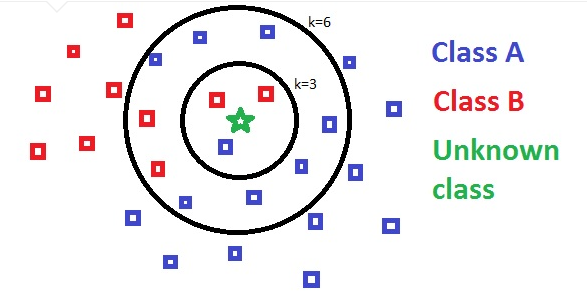
\includegraphics[width=0.8\textwidth]{graphics/knn.png}
  \caption{Example how the choice of $k$ changes the classification of an event. With $k=3$ the unknown event is classified to class B and with $k=6$ it is classified as class A \cite{kNN}.}
  \label{fig:knn}
\end{figure}


\subsection{Quality Parameters}
The quality of the separating power of a classifier is evaluated by different quality parameters.
The first two parameters are the purity and the efficiency of the data set:

\begin{align*}
    \text{purity}\, \, p &= \frac{tp}{tp + fp} \\
    \text{efficiency}\, \, r &= \frac{tp}{tp + fn} \, .\\
\end{align*}

The value $tp$ (true-positive) means that a signal event was correctly classified as a signal event while $fp$ (false-positive) means that a background event was falsely classified as a signal event.
Similarly $fn$ (false-negative) means that a signal event was falsely classified as a background event.

The Jaccard index is a value describing how stable the chosen attributes are against statistical fluctuations.
The value is calculated like this:

\begin{equation*}
    J \left(F_a, F_b \right) = \frac{|F_a \cup F_b|}{|F_a \cap F_b|}
\end{equation*}

This is describing how similar the two sets $F_a$ and $F_b$ are.
To describe how stable a dataset is the following calculation is used:

\begin{equation*}
    \hat{J} = \frac{2}{l \left(l - 1 \right)} \sum\limits_{i = 1}^{l}\sum\limits_{j = i+1}^{l} J\left(F_i, F_j \right) \, .
\end{equation*}

It means that the attribute selection is been used $l$ times on $l$ subsets of the dataset.
A value near 1 means that the dataset is stable for statistical fluctuation.

\subsection{Crossvalidation}
To check if a classifier did not implement statistical fluctuations the dataset is divided into $n$ subsets.
The classifier is trained on $n-1$ of these subsets and then tested on the remaining subset.
This method will be repeated $n$ times so that every subset is used as a test subset once.
The resulting $n$ values for purity and efficiency are taken into average.

\subsection{ROC curves}
A reciever operator curve (ROC curve) shows the ratio of \textit{true positives} against \textit{false positives}.
A straight line between $\left(0,0 \right)$ and $\left(1,1 \right)$ represents a model with total random classification since for every value of the classification the same number of true positive and false positive events is given.
A perfect classification would be shown in a curve that goes straight up to the top left corner and then to the top right corner.
According to that the area under the curve (ROC AUC score) is a metric that shows the separation power of a classifier.
A ROC AUC of $0.5$ corresponds to a total random classification while a ROC AUC near $1$ is showing a good separation power.
